\documentclass[oribibl]{llncs}
%
\usepackage{framed}
\usepackage{array}
\usepackage{multirow}
\usepackage{graphicx}

\begin{document}

\title{Automatic Acquisition of Controlled Vocabularies from Wikipedia using Wikilinks, Word Ranking, and a Dependency Parser}

%\author{Ruben Dorado\inst{1} \and Audrey Bramy\inst{1} \and Camilo Mej\'ia-Moncayo\inst{2} \and Alix E. Rojas\inst{2}}

%\institute{
%\'Ecole de technologie sup\'erieure, Universit\'e du Qu\'ebec, Montreal, %Canada\\
%\email{ruben.dorados, audrey.bramy@gmail.com} 
%\and
%Universidad EAN, Bogot\'a, Colombia\\
%\email{cmejiam,aerojash@universidadean.edu.co}
%}

\maketitle

\begin{abstract}
Controlled vocabularies are important resources used in several tasks such as machine translation, text summarization, and text analysis. However, the development of such resources is expensive and time-consuming. On the other hand, the Wikipedia, a free collaborative encyclopedia, contains plenty of semi-structured information that can be used by an automatic process to create new resources. This paper proposes a method to extract semantic information from the Wikipedia in the form of a controlled vocabulary. The method combines keywords obtained for a specific Wikipedia article with three different strategies: using Wikipedia annotations called wikilinks, a ranking measure to obtain keywords from text, and a dependency parser. To evaluate the model, we performed an analysis in terms of coverage and performance of the acquired vocabulary using WordNet as a gold standard. 
\end{abstract}


\section{Introduction}

Wikipedia is a free-access encyclopedia, written by all people over the world. Wikipedia is targeted to a general public that can collaborate by improving its content through a web interface. Users of Wikipedia edit the content by adding new text that includes annotations with information such as links between articles and categories. These annotations turn a Wikipedia article into a complex semantic network of inter-related terms.

Wikipedia's articles contain different sort of metadata annotations: content tables, categories, inter-language links, and Wikipedia markup annotations in the text such as links to internal pages, called freelinks. That information has been used previously for knowledge discovery using the Wikipedia. Some examples include mining information from content tables or Wiki infoboxes \cite{Lin2011}, taxonomy deriving from Wiki categories \cite{Zesch2007}, and topic hierarchies from Wiki categories \cite{Hu2015}.

In this study, we analyze the use of a Wikipedia to obtain a set of keywords given a specific article. We explore three different methods to acquire semantic related words. Such set of keywords can be seen as an entry in a semantic dictionary or a controlled vocabulary, where the title of the Wikipedia article is the concept and the terms related to the concept are the keywords. We argue that such set of semantically related keywords can be useful in many scenarios, such as text classification where they can be used as the features for a classifier to reduce the dimensionality. We propose to acquire a set of words is, in fact, a controlled vocabulary, where the name of the article is the main term and text and annotations on the article contain the edges to other nodes. For example, given a set of terms such as {\it Christianity}, {\it Bible}, {\it Computer}, and {\it Operating system}, it is possible to acquire a set of related terms for each of those articles. This controlled vocabulary can be used for different tasks like text classification, where each of the terms is related to one of the following categories: {\it Religion} or {\it Computers}. Then, the categorized vocabulary can be used as feature reduction method to classify the documents, reducing the time an usual method need to analyze a document since the possible set of features is being reduced.  

In this study, we focus on using three different methods to obtain keywords from a specific Wikipedia article. The first one is using annotations to other articles in a Wikipedia article called wikilinks. The second one is extracting keywords from the text taking into account the frequency of the term in the article. The thirds one is also using the text to find syntactic relations between a particular term in the sentences. Finally, we propose a method to combine them all, improving the precision of the quality set of keywords.


We experimented with the information provided by a set of specific articles and compared the results with the well know resource called WordNet. WordNet organizes terms as a group of synonyms called synset, similar to a thesaurus. We used WordNet to measure the quality of the acquired set of words for each article by comparing it with the terms found on the WordNet synset. 

The rest of this article is explained as follows. Section 2 provides information about the related work in information extraction using the Wikipedia. Section 3 contains an explanation of the three methods used to extract keywords. Empirical results are presented and discussed in section 4, while section 5 presents the conclusions.    

\section{Related works}

Recently, Wikipedia has been used as a source of information. To give some examples, \cite{Mihalce2007} describes a method to obtain semantic information for word sense disambiguation. \cite{Makris2013} presents a system that trains himself with data from Wikipedia to perform text annotation and add semantic information to plan texts. \cite{Garcia2011} extracts taxonomies from Wikipedia. Other works have proved that information such as hyperlink relations between a set of documents \cite{Davison2000} can be used to obtain a set of interrelated terms. Another kind of studies have used hyperlinks in the Wikipedia provides more information than in a common website \cite{Nakayama2007}. 

Dependency parsing has proven to be a method to acquire semantic patterns because they are capable of representing relations between elements of a sentence. For example, a dependency parser has been used to infer rules for automatic question answering \cite{Lin2001} and paraphrase identification \cite{Szpektor2004}. Generally, these systems have been focused on relation extraction, the identification of particular relations between items in the text. The relations used and the method to acquire them vary across studies. For example, \cite{Yangarber2003} used an [s,v,o] (subject, verb, direct object) tuples as patterns while \cite{Sudo2001} allow any analysis to be a possible pattern. Machine learning algorithms are also used to learn and identify instances of relations such as iterative semi-supervised algorithms \cite{Greenwood2006} where usually the algorithm is provided with an initial set of patterns and attempts to increase the number of patterns and relations between items. This work, however, is more related to the work of \cite{Sudo2001,Stevenson2009}, in the sense it uses different sources to rank terms obtained by a dependency parser. \cite{Sudo2001} used tf-idf method to rank patterns according to where they tended to occur in documents which were known to contain information of interest while \cite{Stevenson2009} proposed a ranking term measure to give a value to terms obtained by patterns obtained from the result of a dependency parser. 
 
%\cite{Mihaltz2010}


\section{Acquiring a Controlled Vocabulary from Wikipedia}


This section describes the proposed process to acquire a controlled vocabulary from the Wikipedia. First, we describe the general process to acquire a set of keywords related to a specific article using three approaches and then mixing them. Then, we explain each one of the three approaches: wikilinks, word ranking, and dependency parsing. 

We define a controlled vocabulary as a list of concepts, also called entries, where each of them has selected list of words semantically related to such concept. A controlled vocabulary provides a method to organize knowledge. It is used in subject indexing schemes, subject headings, thesauri, taxonomies and other forms of knowledge organization systems. A controlled vocabulary specifies the use of terms and phrases related to a concept, similar to a dictionary, where each of the entries has a set related terms. In this case, we are interested in acquiring only the terms related to a concept. For example, given the concept 'cat', the task is to acquire a set of words that are related such as 'animal', 'eat', or 'kitty'. 

We propose to acquire a controlled vocabulary for specific terms using articles from the Wikipedia. Figure \ref{fig:extraction} depicts the extraction process. Having an article from Wikipedia, two different extraction processes are performed: extraction of terms using wikilinks (1) and text extraction (2). Extraction of terms using wikilinks is explained in detail in Section \ref{subsec:wikilinks}, while text extraction consists in extracting the text of the article. Extraction of terms using term frequency (3) and a dependency parser (4) is performed on the extracted text. Both processes are explained in Section \ref{subsec:frequency} and Section \ref{subsec:parsing} respectively. Finally, the three set of keywords is combined to finally obtain one set of keywords (5). The combination process is explained in Section \ref{subsec:mixing}.

\begin{figure}[t]
\centering
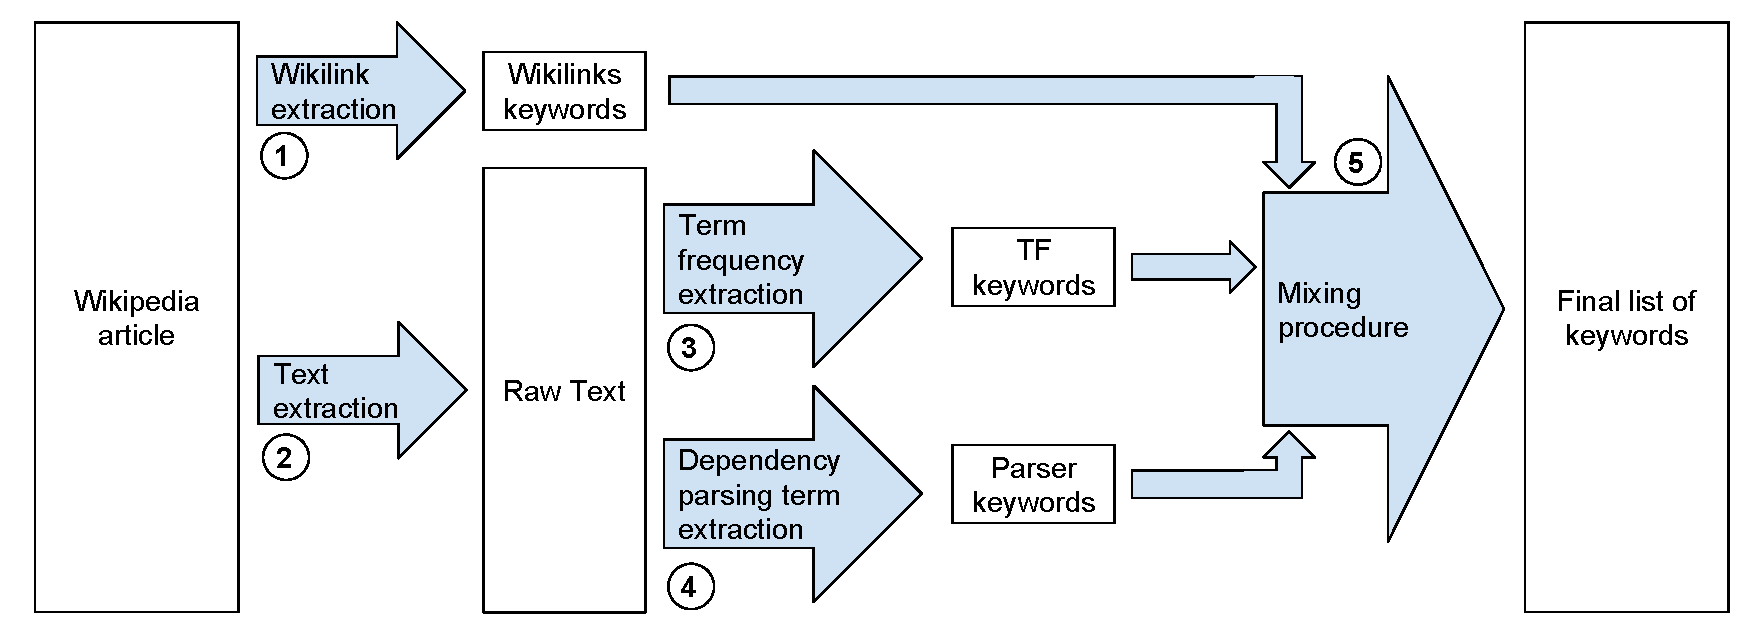
\includegraphics[height=4.5cm]{images/extraction}
\caption{Pipeline of the proposed method to extract the controlled vocabulary.}
\label{fig:extraction}
\end{figure}


\subsection{Extraction of terms using Wikilinks} \label{subsec:wikilinks}

The structure of Wikipedia can be exploited in several ways. In particular, we are interested in using the so-called {\it wikilinks}. A wikilink is a reference to different Wikipedia article. For example, the following wikitext has been extracted from the article {\it Operating system}: 

\begin{center}
\fbox {
    \parbox{0.8\linewidth}{
Examples of popular desktop operating systems include \texttt{[[Apple Inc.\textbar Apple]] [[OS X]], [[Linux]]} and its variants, and \texttt{[[Microsoft Windows]]}. So-called \texttt{[[mobile operating system]]}s include \texttt{[[Android (operating system)\textbar Android]]} and \texttt{[[iOS]]}.}}
\end{center}

It can be seen in the above example that it is possible to extract valuable keywords such as {\it Linux}, {\it Microsoft Windows}, and {\it Android}, represented by wikilinks. Furthermore, this information can be easily extracted since wikilinks maintain a regular pattern in the source of the article. One of the questions addressed in this article is how much of this information provided by all the wikilinks of a specific article is closely related to the semantic meaning of the article. 

\subsection{Term acquisition using frequency ranking} \label{subsec:frequency}

Frequency word ranking has been used to distinguish important terms in texts under the assumption that the importance of a term that occurs in a document is proportional to its term frequency. In other words, a term that frequently appears in the text is supposed to be important. The frequency of a term $t$ in a document $a$, in this case, a Wikipedia article, is calculated as follows:
\[
f(t,a) = f_{t,a} = count(t, a),
\]where the $count(t, a)$ is number of times the term $t$ occurs in the document $a$.

However, in cases where the length of documents vary adjustments and normalizations are often made. We use the following measures to evaluate the usefulness of a term $t_i$:

\begin{itemize}
\item{Term Frequency score (TF) : \[\frac{f_{t,a}}{ \max\{ f_{t',a} : t' \in a \} },\]where $f_{t,a}$ is the number of times the term $t$ appears on the article $a$.}
\item{Scaled Term Frequency score (STF) : \[(1-k) + k\frac{f_{t,a}}{ \max\{ f_{t',a} : t' \in a \} },\]where $f_{t,a}$ is the number of times the term $t$ appears on the article $a$ and $k \in R^+, 0 < k \leq 1 $.}
\item{Log-scaled Term Frequency score (LTF): \[ \frac{\log(f_{t,a}) }{\log(\max\{ f_{t',a} : t' \in a \})}\]}
\end{itemize}
 
The term frequency score is the normalized count of the terms, where the value of term that occurs the most is 1 and a non important term in the document is close to 0. The scaled term frequency score provides a method to change the minimum weight of the frequency score using the $k$ parameter. In other words, the STF score transforms any given value of the TF score from the range $[0,1]$ to $[k,1]$. The scale is  $k$ equal to 0.5. Finally, the log-scaled term frequency score allows to normalize a given value penalizing low occurrences. It worth mentioning that the normalized and scaled scores only work when combining the scores with other functions or to compare ranked works in different documents. If the purpose is to extract words in a document, the transformations will not help since they are all monotonic functions.

\subsection{Dependency parsing} \label{subsec:parsing}

A dependency parser is a computational tool that takes a sentence as input and returns a tree, called a parse tree, that contains connections between words according to their relationships. In the tree, each node represents a word, child nodes are words that are dependent on the parent, and edges are labeled according to the relationship between the parent an the child. The set of relationships depends on the grammar. For example, The Universal Dependencies (UD) project defines a set of relations that by developing cross-linguistically treebank annotation for several languages \cite{Nivre2016}. Under such grammar, there is a relation called {\it nsubj} between two words $w1 \to w2$ that represents the case when $w2$ is a noun that is the syntactic subject of the clause. As an example, in the phrase 'Colombia won the tournament', the word ´´Colombia' is related to the verb 'won' through the relation {\it nsubj}. Figure \ref{fig:depex} shows the result of the parse tree of such sentence.


\begin{figure}[h]
\centering
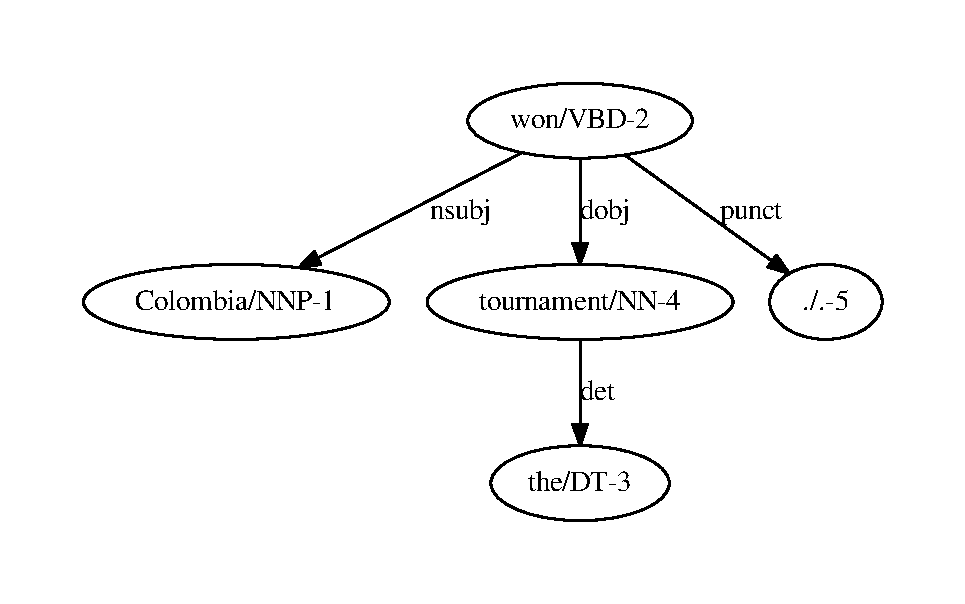
\includegraphics[height=4.5cm]{images/depex}
\caption{An example of the dependency tree for the sentence 'Colombia won the tournament'.}
\label{fig:depex}
\end{figure}

We propose the use of three relations to consider possible terms as candidates: 

\begin{itemize}
\item Any word that is the dominant of a nominal subject (nsubj) and is a verb and is related to the target concept. In Figure \ref{fig:depex} the word 'won' would be selected. The objective of this relation is to find verbs.
\item Any word that is a noun, has a dominant relation of any type with another node $m$, and $m$ is the target concept. In Figure \ref{fig:depex} the word 'tournament' would be selected. The objective of this relation is to find nouns.  
\item Any word that is a noun and also has dominant relation of any type  with any node. The objective of this relation is also to find nouns.
\end{itemize}


\subsection{Mixing sets of terms} \label{subsec:mixing}

The last part of the proposed method consists of combining the three previous methods to obtain keywords into one. We propose such combination by transforming each of the three previous methods into a normalized score and using a set of mixing coefficients, one for each of the scores. In the case of keywords extracted using the wikilink approachx, we propose the usage of an indicator function $WL(t,a)$ that returns 1 if the article $a$ contains a wikilink with the term $t$ and 0 if it does not. For the term frequency score for a particular document $WF(t,a)$, we propose the use one of the scores defined in Subsection \ref{subsec:frequency}. For the third one, the dependency parser usage, we also propose to use an indicator function $DP(t, a)$ that returns 1 if any of the relations listed in Section \label{subsec:parsing} regarding the term $t$ is found in the article $a$ and 0 if it does not. Finally, a set of mixing coefficients $\alpha$, $\beta$, and $\gamma$ are used to control the importance of each score. The formal mathematical definition is stated as follows:   

\[
rank(t,a) = \alpha WL(t,a) + \beta WF(t,a) + \gamma DP(t,a),
\]where $\alpha \in R^+$, $\beta \in R^+$, and $\gamma \in R^+$, $\alpha + \beta + \gamma = 1$, are the mixing coefficients, $WL(t, a)$ is wikilinks indicator score, $WF(t,a)$ is a word frequency score, and $DP(t,a)$ is the dependency score.

\subsection{Evaluation measures} \label{subsec:eval}

In order to test the performance of our method, we propose the use of {\it precision} and {\it recall} measures. More specifically, given this set of target terms for a specific article $S = \{s_1,s_2,...,s_K\}$, the precision of a set of terms $T_a = \{t_1,t_2,...,t_N\}$ obtained for an article $a$ related to $S$ is calculated as:
\[
precision(T_a) = \frac{count(\{t' \in S\})}{N},
\] 
the recall as:
\[
recall(T_a) = \frac{count(\{t' \in S\})}{K},
\] 
and F1 score as:
\[
F1score(T_a) = 2*\frac{precision*recall}{precision + recall}
\]

\section{Experimentation and results}

We used the Wikipedia dump, which is a file containing all the information stored in the Wikipedia in a specific time. To test our method, we used the also publicly available and well-known resource WordNet. WordNet organizes terms as a group of synonyms called synset. Each entry is called a synset and can be acquired using its surface word similar to a thesaurus. We used WordNet to measure the quality of the acquired set of words. For each selected article, we searched for all the possible terms that belong to the synset and that also are in the article. For example, given the article 'Sport', we included the term 'champion' if it is found in the Wikipedia article and also in the WordNet synset for 'sport'.  

There are different measures to obtain synsets in the Wikipedia. We selected its the top terms using Wu-Palmer Similarity (WUP) \cite{Wu1994} and Leacock-Chodorow Similarity (LCS) \cite{Leacock1998} with a threshold of 0.7. Finally, we used precision, recall, and F1 scores to evaluate the performance of the different strategies, as described in Subsection \ref{subsec:eval}. 

For experimentation, we selected manually 18 articles. Each article was pre-processed to extract all the information described previously: the set of wikilinks and text from a set of preselected articles. We used the publicly available library {\it wikitools} to extract the text and wikilinks from a set of articles\footnote{The library can be found the in the git repository: https://github.com/rdorado79/wikitools}. With the text, we removed stopwords, punctuation, and transformed the text to lower case. Then, we selected two set keywords for each article using term frequency and a dependency parser. We used the Stanford Dependency Parser \cite{Klein2003} as dependency parser in our experimentation. Finally, we measured how many of these terms are in the selected subset of terms from its WordNet synset. 


\begin{table}[t]
\centering
\begin{tabular}{
|m{14mm}
|>{\centering\arraybackslash}m{10mm}
|>{\centering\arraybackslash}m{10mm}
|>{\centering\arraybackslash}m{9mm}
|>{\centering\arraybackslash}m{9mm}
|>{\centering\arraybackslash}m{9mm}
|>{\centering\arraybackslash}m{9mm}
|>{\centering\arraybackslash}m{9mm}
|>{\centering\arraybackslash}m{9mm}
|>{\centering\arraybackslash}m{9mm}
|>{\centering\arraybackslash}m{9mm}|
}
\hline
\multirow{2}{14mm}{\centering\textbf{Concept}}&
\multirow{2}{10mm}{\centering\textbf{Count}}& 
\multicolumn{3}{>{\centering\arraybackslash}m{27mm}|}{\textbf{Wikilinks}}&
\multicolumn{3}{>{\centering\arraybackslash}m{27mm}|}{\textbf{TF-score}}&
\multicolumn{3}{>{\centering\arraybackslash}m{27mm}|}{\textbf{Parser}}
\\ \cline{3-11} 
& & 
\multicolumn{1}{>{\centering\arraybackslash}m{9mm}|}{\textbf{Prec}}& 
\multicolumn{1}{>{\centering\arraybackslash}m{9mm}|}{\textbf{Rec}}&
\multicolumn{1}{>{\centering\arraybackslash}m{9mm}|}{\textbf{F1}}&
\multicolumn{1}{>{\centering\arraybackslash}m{9mm}|}{\textbf{Prec}}& 
\multicolumn{1}{>{\centering\arraybackslash}m{9mm}|}{\textbf{Rec}}&
\multicolumn{1}{>{\centering\arraybackslash}m{9mm}|}{\textbf{F1}}&
\multicolumn{1}{>{\centering\arraybackslash}m{9mm}|}{\textbf{Prec}}& 
\multicolumn{1}{>{\centering\arraybackslash}m{9mm}|}{\textbf{Rec}}&
\multicolumn{1}{>{\centering\arraybackslash}m{9mm}|}{\textbf{F1}}
\\  

\hline

Sport & 177 & 0.083 & 0.107 & 0.094 & 0.155 & \textbf{0.232} & \textbf{0.186} & \textbf{0.313} & 0.028 & 0.052 \\
Religion & 128 & 0.076 & \textbf{0.320} & 0.123 & 0.120 & 0.180 & \textbf{0.144} & \textbf{0.185} & 0.094 & 0.124 \\
Baseball & 29 & 0.016 & \textbf{0.276} & 0.031 & \textbf{0.093} & 0.138 & \textbf{0.111} & 0.051 & 0.103 & 0.068 \\
Soccer & 9 & 0.025 & \textbf{0.667} & 0.049 & 0.308 & 0.444 & \textbf{0.364} & \textbf{0.400} & 0.222 & 0.286 \\
CPU & 34 & 0.009 & 0.059 & 0.016 & \textbf{0.078} & \textbf{0.118} & \textbf{0.094} & 0.068 & 0.088 & 0.077 \\
Horse & 95 & 0.070 & \textbf{0.305} & 0.114 & 0.056 & 0.084 & 0.068 & \textbf{0.153} & 0.095 & \textbf{0.117} \\
Country & 46 & 0.136 & 0.174 & 0.152 & \textbf{0.159} & \textbf{0.239} & \textbf{0.191} & 0.125 & 0.022 & 0.037 \\
Computer & 114 & 0.045 & \textbf{0.158} & 0.071 & 0.094 & 0.140 & \textbf{0.112} & \textbf{0.109} & 0.053 & 0.071 \\
God & 108 & 0.074 & \textbf{0.278} & 0.117 & 0.117 & 0.176 & \textbf{0.141} & \textbf{0.189} & 0.093 & 0.124 \\
Dog & 141 & 0.044 & 0.099 & 0.061 & 0.076 & \textbf{0.113} & 0.091 & \textbf{0.164} & 0.071 & \textbf{0.099} \\
Planet & 66 & 0.064 & \textbf{0.379} & 0.109 & 0.172 & 0.258 & \textbf{0.206} & \textbf{0.200} & 0.167 & 0.182 \\
Jehovah & 31 & 0.032 & \textbf{0.226} & 0.055 & \textbf{0.065} & 0.097 & \textbf{0.078} & 0.036 & 0.032 & 0.034 \\
Music & 269 & 0.093 & \textbf{0.294} & 0.141 & 0.141 & 0.212 & \textbf{0.170} & \textbf{0.261} & 0.112 & 0.156 \\
Canada & 35 & 0.013 & \textbf{0.257} & 0.024 & \textbf{0.038} & 0.057 & 0.046 & 0.036 & 0.086 & \textbf{0.050} \\
Animal & 171 & \textbf{0.132} & \textbf{0.234} & \textbf{0.169} & 0.070 & 0.105 & 0.084 & 0.000 & 0.000 & NaN \\
Colombia & 29 & 0.016 & \textbf{0.448} & 0.030 & 0.070 & 0.103 & 0.083 & \textbf{0.111} & 0.207 & \textbf{0.145} \\
Cat & 106 & 0.051 & \textbf{0.198} & \textbf{0.082} & 0.038 & 0.057 & 0.045 & \textbf{0.060} & 0.028 & 0.038 \\
Japan & 61 & 0.016 & \textbf{0.180} & 0.029 & 0.055 & 0.082 & 0.066 & \textbf{0.059} & 0.082 & \textbf{0.068} \\

 \hline
 Average & 91.61 & 0.055 & {\bf0.259} & 0.081 & 0.106 & 0.157 & {\bf 0.127} & {\bf 0.140} & 0.088 & 0.096\\
 \hline
\end{tabular}
\caption{Results of the experimentation in counts}
\label{table:1}
\end{table}

For the experimentation, we selected a set of 18 articles. The full list can be seen in Table \ref{table:1}, along with the results. The first column shows the name of the article. The second column shows the number of targeted words for the specific article. Columns 3 to 5 show the results for wikilinks, 6 to 8 for term frequency, and columns 9 to 11 for the dependency parser. It can be concluded that Wikilink term extraction gives the best recall between the three methods. This suggests that the keywords obtained using the wikilinks contain similar semantic information to  Wordnet. In terms of precision, the keywords obtained by the dependency parser strategy seem to correlate WordNet slightly better. However, the best F1-score on average is obtained by the keywords obtained using the term frequency measure.    


\begin{table}[t]
\centering
\begin{tabular}{
|m{14mm}
|m{33mm}
|m{33mm}
|m{33mm}|
}
\hline
\multicolumn{1}{|>{\centering\arraybackslash}m{14mm}|}{\textbf{Concept}}& 
\multicolumn{1}{>{\centering\arraybackslash}m{33mm}|}{\textbf{Wikilinks}}&
\multicolumn{1}{>{\centering\arraybackslash}m{33mm}|}{\textbf{TF score}}& 
\multicolumn{1}{>{\centering\arraybackslash}m{33mm}|}{\textbf{Dependency }}
\\  

\hline

Sport & competitive, physical activity, game, entertainment, tie-breaking methods, tournament, champion, playoffs & participants, physical, participation, used, including, competition, increase, football, international, games & charter, technology, participation, venue, popularity, definition, set, noun, running, spectator, football\\ 
\hline
Religion & cultural system, behaviors, world view, sacred texts, societal organisation, human, existence, divine & world, one, people, law, study, faith, belief, beliefs, include, sacred, god, defined, science, countries & view, essence, king, edition, violence, absence, excess, influence, part, role, affects, morality, deals, science\\
\hline
CPU & electronic circuit, computer, instruction, computer program, input/output, control unit, main memory, design &  instruction, cpus, clock, instructions, program, memory, data, performance, operation, processors, execution & dissipation, cycle, context, perform, hardware, performance, designs, design, parallelism, operation, execute\\

\hline
Horse & extant, subspecies, equus ferus, mammal, equidae, evolved, eohippus, domesticate, anatomy, colors & breeds, developed, wild, domesticated, bones, four, animals, well, human, age, world & tibia, blood, movement, appears, style, control, rider, breed, pedigree, domestication, remains, zebra, animal\\
\hline
Country & political geography, sovereign state, political division, people, league of nations, united nations, states & country, sovereign, state, word, political, independent, associated, territory, english, govpubs, gov, derived & version, coal, part, sense, name, resident, sovereign state, region\\
 \hline
\end{tabular}
\caption{Random examples of the words extracted for some articles}
\label{table:3}
\end{table}

Despite the relatively low values, a thorough analysis of the extracted word shows encouraging results. Table \ref{table:3} depicts examples of the extracted words for each one of the three methods. It can be seen the nature of the words extracted by each method. Terms extracted from wikilinks tend to be concepts that complement the Wikipedia article since wikilinks are links to other articles. Examples of these are 'tie-breaking' for the article 'Sport', or 'equus ferus' for 'Horse'. Terms extracted using the frequency are generally those that are used to explain important concepts in the document and appear frequently. Examples of these are 'faith' in the article 'Religion' and 'territory' in 'Country'. Finally, terms extracted with the dependency parser are generally functional words related to the concept. For example, the word 'movement' for 'Horse' or the word 'affect' for religion. It worths mentioning that the patterns used were very simple and are susceptible to improvement in many ways. This is left for future work.

The last part of the method to combine all the previous acquired set of words into one unique set. We combined all the three previous strategies by the method proposed in Section \ref{subsec:eval}. Testing with different values for $\alpha$, $\beta$, and $\gamma$, we found that appropriate values for the model are a high $\beta$ and a $\gamma$ value slightly higher than $\alpha$. This is possible due that the TF score is lower than the other two and tend to be ruled out if it is not properly scaled and weighted. Also, a higher $\gamma$ allows preference from the dependency parser, since they have a high precision. 

Table \ref{table:2} shows the results with $\alpha = 0.08$, $\beta = 0.8$, and $\gamma = 0.12$ for the mixing model. We also set $k=0.8$ for the $k$ parameter of the scaled TF score. It can be seen in the table that we successfully combined all the three strategies, wikilinks, term frequency, and the dependency parser, into one method obtaining an increment in the F1-score. It is also difficult to say which of the TF score used is better than other. Numerically, the scaled TF score outperforms the other two but log scaled TF score gives close values to the best found. 


\begin{table}[t]
\centering
\begin{tabular}{
|m{15mm}
|>{\centering\arraybackslash}m{9mm}
|>{\centering\arraybackslash}m{9mm}
|>{\centering\arraybackslash}m{9mm}
|>{\centering\arraybackslash}m{9mm}
|>{\centering\arraybackslash}m{9mm}
|>{\centering\arraybackslash}m{9mm}
|>{\centering\arraybackslash}m{9mm}
|>{\centering\arraybackslash}m{9mm}
|>{\centering\arraybackslash}m{9mm}|
}
\hline
\multirow{2}{*}{\centering\textbf{Concept}} &
\multicolumn{3}{>{\centering\arraybackslash}m{27mm}|}{\textbf{TF score}} & 
\multicolumn{3}{>{\centering\arraybackslash}m{27mm}|}{\textbf{Scaled TF score}} & 
\multicolumn{3}{>{\centering\arraybackslash}m{27mm}|}{\textbf{Log TF score}}\\
\cline{2-10} 
& \multicolumn{1}{>{\centering\arraybackslash}m{9mm}|}{\textbf{Prec}}&
\multicolumn{1}{>{\centering\arraybackslash}m{9mm}|}{\textbf{Rec}}& 
\multicolumn{1}{>{\centering\arraybackslash}m{9mm}|}{\textbf{F1}}&
\multicolumn{1}{>{\centering\arraybackslash}m{9mm}|}{\textbf{Prec}}&
\multicolumn{1}{>{\centering\arraybackslash}m{9mm}|}{\textbf{Rec}}& 
\multicolumn{1}{>{\centering\arraybackslash}m{9mm}|}{\textbf{F1}}&
\multicolumn{1}{>{\centering\arraybackslash}m{9mm}|}{\textbf{Prec}}&
\multicolumn{1}{>{\centering\arraybackslash}m{9mm}|}{\textbf{Rec}}& 
\multicolumn{1}{>{\centering\arraybackslash}m{9mm}|}{\textbf{F1}}
\\  

\hline

Sport & 0.121 & 0.215 & 0.155 & 0.137 & 0.243 & 0.175 & \textbf{0.153} & \textbf{0.271} & \textbf{0.196} \\
Religion & \textbf{0.158} & \textbf{0.227} & \textbf{0.186} & \textbf{0.158} & \textbf{0.227} & \textbf{0.186} & 0.119 & 0.180 & 0.143 \\
Baseball & 0.059 & 0.103 & 0.075 & \textbf{0.136} & \textbf{0.207} & \textbf{0.164} & 0.133 & \textbf{0.207} & 0.162 \\
Soccer & 0.182 & 0.222 & 0.200 & \textbf{0.364} & \textbf{0.444} & \textbf{0.400} & \textbf{0.364} & \textbf{0.444} & \textbf{0.400} \\
CPU & 0.078 & 0.118 & 0.094 & \textbf{0.096} & \textbf{0.147} & \textbf{0.116} & 0.077 & 0.118 & 0.093 \\
Horse & \textbf{0.117} & \textbf{0.179} & \textbf{0.142} & \textbf{0.117} & \textbf{0.179} & \textbf{0.142} & 0.106 & 0.168 & 0.130 \\
Country & 0.169 & 0.283 & 0.211 & \textbf{0.182} & \textbf{0.304} & \textbf{0.228} & 0.141 & 0.239 & 0.177 \\
Computer & 0.081 & 0.123 & 0.098 & 0.089 & 0.140 & 0.109 & \textbf{0.108} & \textbf{0.175} & \textbf{0.134} \\
God & \textbf{0.170} & \textbf{0.241} & \textbf{0.199} & \textbf{0.170} & \textbf{0.241} & \textbf{0.199} & 0.168 & \textbf{0.241} & 0.198 \\
Dog & 0.086 & 0.142 & 0.107 & \textbf{0.091} & \textbf{0.149} & \textbf{0.113} & 0.082 & 0.135 & 0.102 \\
Planet & \textbf{0.212} & \textbf{0.273} & \textbf{0.238} & 0.202 & \textbf{0.273} & 0.232 & 0.196 & \textbf{0.273} & 0.228 \\
Jehovah & 0.053 & 0.065 & 0.058 & 0.053 & 0.065 & 0.058 & \textbf{0.077} & \textbf{0.097} & \textbf{0.086} \\
Music & \textbf{0.170} & 0.227 & 0.194 & \textbf{0.170} & 0.227 & 0.194 & 0.169 & \textbf{0.230} & \textbf{0.195} \\
Canada & 0.063 & \textbf{0.086} & 0.072 & \textbf{0.068} & \textbf{0.086} & \textbf{0.076} & 0.037 & 0.057 & 0.045 \\
Animal & \textbf{0.116} & \textbf{0.187} & \textbf{0.143} & 0.083 & 0.135 & 0.103 & 0.080 & 0.129 & 0.098 \\
Colombia & 0.167 & \textbf{0.207} & 0.185 & \textbf{0.188} & \textbf{0.207} & \textbf{0.197} & 0.150 & \textbf{0.207} & 0.174 \\
Cat & \textbf{0.045} & \textbf{0.075} & \textbf{0.057} & \textbf{0.045} & \textbf{0.075} & \textbf{0.057} & 0.033 & 0.057 & 0.042 \\
Japan & \textbf{0.074} & \textbf{0.115} & \textbf{0.090} & \textbf{0.074} & \textbf{0.115} & \textbf{0.090} & 0.072 & \textbf{0.115} & 0.089 \\

 \hline
  Average & 0.118 & 0.171 & 0.139 & {\bf 0.135} & {\bf 0.192} & {\bf 0.158} & 0.126 & 0.185 & 0.149\\ 
 \hline 
\end{tabular}
\caption{Results of mixing method with $\alpha = 0.08$, $\beta = 0.8$, and $\gamma = 0.12$ and $k=0.8$ for the scaled TF score.}
\label{table:2}
\end{table}


\section{Conclusions}

We presented a method to obtain a set of keywords, called a controlled vocabulary, from Wikipedia articles. The method consists in the combination of other three different methods to obtain keywords: wikilinks, term frequency, and a dependency parser. The presented method successfully combine all the three strategies, wikilinks, term frequency, and the dependency parser, into one achieving an increment in the F1-score. 

In relation with the words extracted from each one of the methods, we can say that they differ substantially. As discussed in the results section, terms extracted from wikilinks tend to be additional concepts that complement the article. Terms extracted using the frequency are keywords that are used to explain important concepts in the document. Finally, terms extracted with the dependency parser are generally functional words related to the concept. 

With respect to the dependency parser, we used three different relations: direct object of the term (dobj) to obtain verbs and two based on nominal subjects (nsubj) to obtain nouns. The method showed to be very promising in terms of precision and it worth improve the patterns in the future.  

We expect to extend this work in many ways. First, we expect to perform a deeper analysis that involves a much higher number of articles. Second, we would like to explore the idea of acquiring automatically grammatical rules for dependency parsing based term acquisition. Third, we would want to perform a deeper analysis on the extraction of keywords using wikilinks. We used a binary function that does not allow to rank and compare words using such method. It would be interesting to propose a rank method for extraction of keywords using wikilinks. 

\bibliographystyle{splncs03}
\bibliography{wiki}


\end{document}
